\documentclass[a4paper,12pt]{report}

\usepackage{geometry}
\geometry{a4paper,left=18mm,right=18mm, top=2cm, bottom=2cm}

\usepackage{lmodern}
\usepackage[T1]{fontenc}
\usepackage[utf8]{inputenc}
\usepackage[ngerman]{babel}
\usepackage[solution_on]{srdp-mathematik} % solution_on/off
\setcounter{Zufall}{0}


\pagestyle{empty} %PAGESTYLE: empty, plain, fancy
\onehalfspacing %Zeilenabstand
\setcounter{secnumdepth}{-1} % keine Nummerierung der Ueberschriften



%
%
%%%%%%%%%%%%%%%%%% DOKUMENT - ANFANG %%%%%%%%%%%%%%%%%%%%%%%%%%%%%%%%%%%%%%%%%%%%%%%%%%%%%%%%%%%%%%%%%%%%%%%%%%%
%
%
\begin{document}
\shorthandoff{"}
\section{104 - AG 1.1, AG-L 2.8, AG 3.1, AG 3.2 - dasd - dasda}

\begin{langesbeispiel}\item[1] %PUNKTE DER AUFGABE
dasd

\antwort{Themen: AG 1.1, AG-L 2.8, AG 3.1, AG 3.2}
\end{langesbeispiel}%
\newpage 
\section{145 - K7 - AG 1.1, AG 1.2, FA 1.1, FA 1.2, DR, DWV - Titel - Quelle}

\begin{langesbeispiel}\item[1] %PUNKTE DER AUFGABE
Text

\antwort{GK/Themen: AG 1.1, AG 1.2, FA 1.1, FA 1.2, DR (7.), DWV (7.)}
\end{langesbeispiel}%
\newpage 
\input{"C:/Users/Chris/Documents/GitHub/Parhamer_connection/Beispieleinreichung/147.tex"}%
\newpage 
\section{AG 1.1 - 10 - Titel juhu - MC - Quelle}

\begin{beispiel}[AG 1.1]{1}
dasdjaöas

\includegraphics{../_database/Bilder/AG11_10_hippo.eps}


dkajjdkajs

\end{beispiel}%
\newpage 
\section{AG 1.1 - 11 - dasdasd - MC - dasdas}

\begin{beispiel}[AG 1.1]{1}
dasdas
\end{beispiel}%
\newpage 
\section{AG 1.1 - 16 - MAT - Zahlen und Zahlenmengen - MC - Matura 2. NT 2017/18}

\begin{beispiel}[AG 1.1]{1}
Nachstehend sind Aussagen über Zahlen und Zahlenmengen angeführt.

Kreuze die beiden zutreffenden Aussagen an!

\multiplechoice[5]{  %Anzahl der Antwortmoeglichkeiten, Standard: 5
				L1={Es gibt mindestens eine Zahl, die in $\mathbb{N}$ enthalten ist, nicht aber in $\mathbb{Z}$.},   %1. Antwortmoeglichkeit 
				L2={$-\sqrt{9}$ ist eine irrationale Zahl.},   %2. Antwortmoeglichkeit
				L3={Die Zahl 3 ist ein Element der Menge $\mathbb{Q}$.},   %3. Antwortmoeglichkeit
				L4={$\sqrt{-2}$ ist in $\mathbb{C}$ enthalten, nicht aber in $\mathbb{R}$.},   %4. Antwortmoeglichkeit
				L5={Die periodische Zahl $1,\dot{5}$ ist in $\mathbb{R}$ enthalten, nicht aber in $\mathbb{Q}$},	 %5. Antwortmoeglichkeit
				L6={},	 %6. Antwortmoeglichkeit
				L7={},	 %7. Antwortmoeglichkeit
				L8={},	 %8. Antwortmoeglichkeit
				L9={},	 %9. Antwortmoeglichkeit
				%% LOESUNG: %%
				A1=3,  % 1. Antwort
				A2=4,	 % 2. Antwort
				A3=0,  % 3. Antwort
				A4=0,  % 4. Antwort
				A5=0,  % 5. Antwort
				}
\end{beispiel}%
\newpage 
\section{AG 1.1 - 17 - das - MC - dasdasas}

\begin{beispiel}[AG 1.1]{1}
dasda
\end{beispiel}%
\newpage 
\section{AG 1.1 - 1[2] - Rationale Zahlen - MC - BIFIE}

\begin{beispiel}[AG 1.1]{1} %PUNKTE DES BEISPIELS
Das ist die ZWEITE Variation der ersten Aufgabe!!!

				Gegeben sind fünf Zahlen.
				
				Kreuze diejenigen beiden Zahlen an, die aus der Zahlenmenge $\mathbb{Q}$ sind!
				\multiplechoice[5]{  %Anzahl der Antwortmoeglichkeiten, Standard: 5
								L1={$0,4$},   %1. Antwortmoeglichkeit 
								L2={$\sqrt{-8}$},   %2. Antwortmoeglichkeit
								L3={$\frac{\pi}{5}$},   %3. Antwortmoeglichkeit
								L4={$0$},   %4. Antwortmoeglichkeit
								L5={$e^2$},	 %5. Antwortmoeglichkeit
								L6={},	 %6. Antwortmoeglichkeit
								L7={},	 %7. Antwortmoeglichkeit
								L8={},	 %8. Antwortmoeglichkeit
								L9={},	 %9. Antwortmoeglichkeit
								%% LOESUNG: %%
								A1=1,  % 1. Antwort
								A2=4,	 % 2. Antwort
								A3=0,  % 3. Antwort
								A4=0,  % 4. Antwort
								A5=0,  % 5. Antwort
								}				
\end{beispiel}
%
\newpage 
\section{AG 1.1 - 21 - ddas - MC - dasdas}

\begin{beispiel}[AG 1.1]{1}
adas
\end{beispiel}%
\newpage 
\section{AG 1.1 - 22 - ljjkjlk - LT - klök}

\begin{beispiel}[AG 1.1]{1}
m.köl
\end{beispiel}%
\newpage 
\section{AG 1.1 - 23 - xasdsa - LT - xsadas}

\begin{beispiel}[AG 1.1]{1}
cxycyxc
\end{beispiel}%
\newpage 
\section{AG 1.1 - 3[1] - Ganze Zahlen - MC - Quelle}

\begin{beispiel}[AG 1.1]{1}
neue variation
\end{beispiel}%
\newpage 
\section{AG 1.1 - 8 Abgeschlossene Zahlenmengen - MC - MK}

\begin{beispiel}[AG 1.1]{1} %PUNKTE DES BEISPIELS
				Eine Zahlenmenge M heißt abgeschlossen bezüglich der Addition (Multiplikation), wenn die Summe (das Produkt) zweier Zahlen aus M wieder in M liegt. Welche der folgenden Mengen sind abgeschlossen gegenüber der Addition? Kreuze die entsprechende(n) Zahlenmenge(n) an.\\

\multiplechoice[5]{  %Anzahl der Antwortmoeglichkeiten, Standard: 5
				L1={$\mathbb{Z}^{+}$},   %1. Antwortmoeglichkeit 
				L2={$\mathbb{Q}$},   %2. Antwortmoeglichkeit
				L3={$\mathbb{N}_{g}$},   %3. Antwortmoeglichkeit
				L4={$\mathbb{R}^{+}$},   %4. Antwortmoeglichkeit
				L5={$[0;1]$},	 %5. Antwortmoeglichkeit
				L6={},	 %6. Antwortmoeglichkeit
				L7={},	 %7. Antwortmoeglichkeit
				L8={},	 %8. Antwortmoeglichkeit
				L9={},	 %9. Antwortmoeglichkeit
				%% LOESUNG: %%
				A1=1,  % 1. Antwort
				A2=2,	 % 2. Antwort
				A3=3,  % 3. Antwort
				A4=4,  % 4. Antwort
				A5=0,  % 5. Antwort
				}
\end{beispiel}%
\newpage 
\section{AG 3.5 - 10 - Titel - OA - Quelle}

\begin{beispiel}[AG 3.5]{1}
Text
\end{beispiel}%
\newpage 
\section{AG-L 1.3 - 1 - K5 - Klavierspielende Mädchen - OA - MatKon}

\begin{beispiel}[AG-L 1.3]{1}
$M$ sei die Menge aller Mädchen einer bestimmten Schulklasse und $K$ die Menge aller Schüler und Schülerinnen dieser Klasse die gerne Klavier spielen.

Beschreibe die folgende Verknüpfung von Mengen in Worten:\leer

$M\cap K=\antwort[\rule{3cm}{0.3pt}]{\text{Die Menge aller Klavier spielenden Mädchen dieser Klasse.}}$
\end{beispiel}%
\newpage 
\section{AG-L 3.6 - 1[1] - K5 - Winkel zwischen Vektoren - OA - eqweqwqe}

\begin{beispiel}[AG-L 3.6]{1}
eqweqweqweqw
\end{beispiel}%
\newpage 
\section{DR - 3 - adasdas - MC - dada}

\begin{beispiel}[DR]{1}
dasdad
\end{beispiel}%
\newpage 
\section{K6 - FO - 3 - Titel - OA - Quelle}

\begin{beispiel}[FO (6.)]{1}
kdööasl dlaskaös
\end{beispiel}%
\newpage 
\section{K1 - BZ.as - 15 - Titel - OA - Quelle}

\begin{langesbeispiel} \item[1] %PUNKTE DES BEISPIELS
Test Test
\end{langesbeispiel}%
\newpage 
\section{K1 - BZ.as - 16 - Titel - MC - dasda}

\begin{langesbeispiel} \item[1] %PUNKTE DES BEISPIELS
TEST
\end{langesbeispiel}%
\newpage 
\section{K1 - BZ.as, BZ.ef, BZ.ek - 20 - dasd - MC - dadas}

\begin{langesbeispiel}\item[1] %PUNKTE DER AUFGABE
dasda

\antwort{Themen: BZ.as (1.), BZ.ef (1.), BZ.ek (1.)}
\end{langesbeispiel}%
\newpage 
\section{78 - MAT - AG 2.4, AN 4.2, AN 4.3, FA 1.4, FA 1.7, FA 3.2, FA 4.1, FA 5.6, WS 1.1, WS 1.2 - Einkommensverteilung - BIFIE Aufgabensammlung}

\begin{langesbeispiel} \item[0] %PUNKTE DES BEISPIELS
	
Der Statistiker Max Lorenz beschrieb bereits im Jahr 1905 statistische Verteilungen mithilfe der nach ihm benannten Lorenz-Kurve. Eine Lorenz-Kurve $f$ kann z.B. zur Beschreibung er Einkommensverteilung in einem Staat herangezogen werden. Je ausgepr�gter ihr "`Bauch"' ist, desto gr��er ist der Einkommensunterschied zwischen niedrigem und hohem Einkommen.

Die Lorenz-Kurve der Einkommensverteilung eines Staates, in dem alle Personen bis auf eine Person nichts verdienen und diese eine Person alles bekommt, wird in der nachstehenden Grafik durch die punktrierten Linien (Katheten eines rechtwinkeligen Dreiecks) dargestellt. Das andere Extrem ist ein Staat, in dem alle Personen gleich viel verdienen. In diesem Fall die die Lorenz-Kurve zu einer Geraden $h$, welche durch die strichlierte Linie dargestellt ist. Zwischen den beiden Extremen verl�uft die Lorenz-Kurve $f$ eines Staates.\leer

Jeder Punkt $P=(x|f(x))$ auf der Kurve $f$ steht f�r folgende Aussage: Die einkommensschw�chsten $x$\,\% aller Haushalte beziehen $f(x)$\,\% des Gesamteinkommens."'

\begin{center}
	\resizebox{0.7\linewidth}{!}{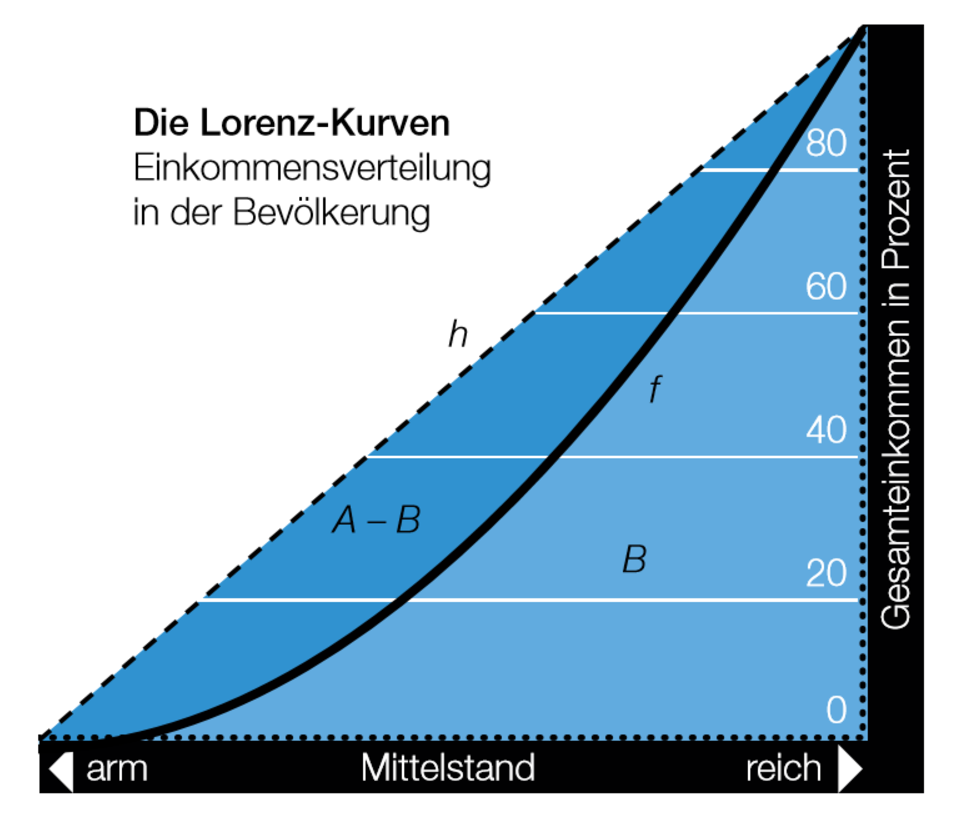
\includegraphics{../Bilder/Bild78-1.eps}}
\end{center}

Der Fl�cheninhalt des rechtwinkligen Dreiecks wird mit $A$ bezeichnet. Der Graph der Lorenz-Kurve $f$ schlie�t mit den beiden Katheten des rechtwinkeligen Dreiecks eine Fl�che mit Inhalt $B$ ein. Setzt man den Inhalt der Fl�che zwischen der Lorenz-Kurve $f$ und der Geraden $h$ mit der Dreiecksfl�che $A$ in Bezug, erh�lt man den Gini-Ungleichheitskoeffizienten $GUK=\frac{A-B}{A}$, eine Zahl zwischen null und ein. Je kleiner der GUK ist, desto gleichm��iger ist das Gesamteinkommen auf die Bev�lkerung verteilt.\leer

In der nachstehenden Grafik ist die Einkommensverteilung in �sterreich in Prozent der gesamten Bruttobez�ge im jahr 2006 dargestellt. Daraus ist z.B. abzulesen, dass jene 20\,\% der Bev�lkerung mit den niedrigsten Bruttoeinkommen nur 2,2\,\% des Gesamtbruttoeinkommens erhalten haben.

\begin{center}
	\resizebox{0.8\linewidth}{!}{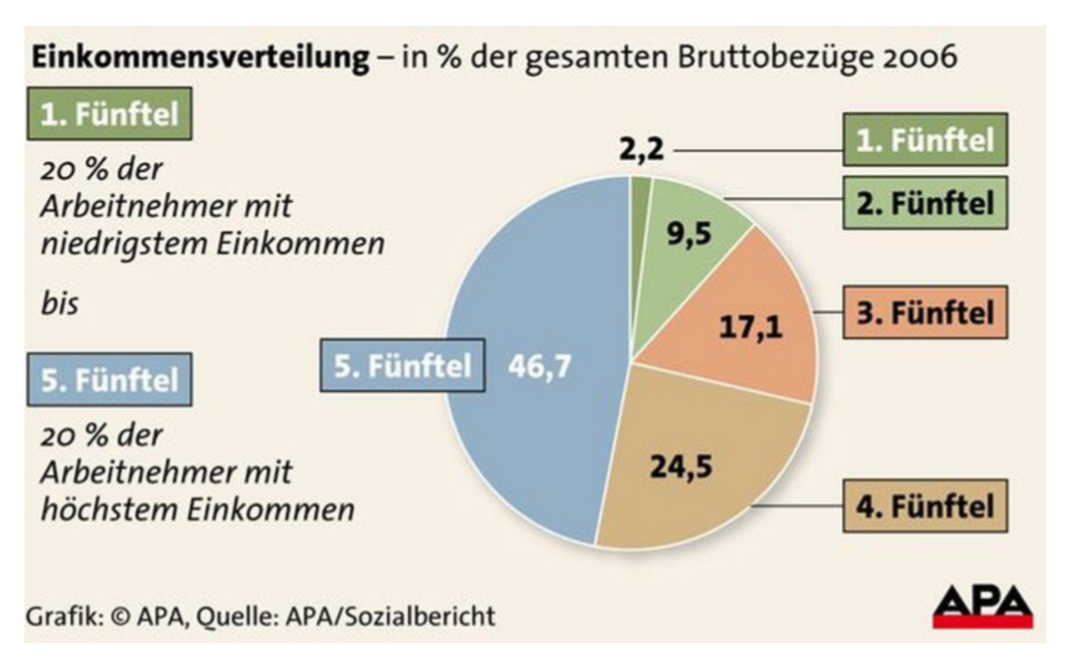
\includegraphics{../Bilder/Bild78-2.eps}}
\end{center}

\begin{scriptsize}\begin{singlespace}Quelle: http://diepresse.com/home/wirtschaft/economist/446997/Sozialbericht\_Einkommen-in-Oesterreich-ungleicher-verteilt [04.05.2017].\end{singlespace}\end{scriptsize}

\subsection{Aufgabenstellung:}
\begin{enumerate}
	\item Zeichne die Lorenzkurve f�r die Einkommensverteilung der Bruttobez�ge in �sterreich im Jahr 2006 in den nachstehenden Grafik als Streckenzug ein!
	
	\begin{center}
		\resizebox{0.8\linewidth}{!}{\psset{xunit=8.0cm,yunit=8.0cm,algebraic=true,dimen=middle,dotstyle=o,dotsize=4pt 0,linewidth=0.8pt,arrowsize=3pt 2,arrowinset=0.25}
\begin{pspicture*}(-0.08726875556452825,-0.12333898008375876)(1.1526748130814817,1.0658128492748549)
\multips(0,0)(0,0.1){12}{\psline[linestyle=dashed,linecap=1,dash=1.5pt 1.5pt,linewidth=0.4pt,linecolor=lightgray]{c-c}(0,0)(1.1526748130814817,0)}
\multips(0,0)(0.2,0){7}{\psline[linestyle=dashed,linecap=1,dash=1.5pt 1.5pt,linewidth=0.4pt,linecolor=lightgray]{c-c}(0,0)(0,1.0658128492748549)}
\psaxes[labelFontSize=\scriptstyle,xAxis=true,yAxis=true,Dx=0.2,Dy=0.1,ticksize=-2pt 0,subticks=2]{->}(0,0)(0.,0.)(1.1526748130814817,1.0658128492748549)
\begin{scriptsize}
\rput[tl](0.023837298973644686,1.0368091461197668){Einkommensanteil (relativ)}
\rput[tl](0.5727012083922189,0.05068323884677006){Einkommensgruppe (Anteil relativ)}
\psline[linewidth=1.2pt,linestyle=dashed,dash=1pt 1pt](0.,0.)(1.,1.)
\rput[tl](0.5660348451199285,0.6275346682646341){h}
\psline[linewidth=1.2pt]{->}(0.7,-0.09)(0.89,-0.09)
\psline[linewidth=1.2pt]{->}(0.49,-0.09)(0.3,-0.09)
\rput[tl](0.49937121239702476,-0.07983342535112656){Mittelstand}
\rput[tl](0.92,-0.075){reich}
\rput[tl](0.2,-0.07983342535112656){arm}
\end{scriptsize}
\end{pspicture*}}
	\end{center}
	
	Berechne mithilfe des eingezeichneten Streckenzuges den GUK f�r die Bruttobez�ge in �sterreich f�r das Jahr 2006!\leer
	
	\item Die Verteilung der Bruttoeinkommen in �sterreich im Jahr 2006 soll durch eine Polynomfunktion $p$ so modelliert werden, dass alle Daten, die aus dem Kreisdiagramm aus der Einleitung abgelesen werden k�nnen mit Funktionswerten dieser Polynomfunktion �bereinstimmen.\leer
	
	Begr�nde, welchen Grad die Polynomfunktion $p$ bei konkreter Berechnung (maximal) hat!\leer
	
	Begr�nde, warum eine Exponentialfunktion $e$ mit $e(x)=a\cdot b^x (a,b\in\mathbb{R}^+$ nicht f�r die Modellierung einer Lorenz-Kurve geeignet ist!\leer
	
	\item Um politische Ma�nahmen absch�tzen zu k�nnen, werden verschiedene Szenarien entworfen. So soll beispielsweise f�r die Bruttoeinkommen langfristig eine Lorenz-Kurve angestrebt werden, die durch die Funktion $g$ mit der Funktionsgleichung $g(x)=0,245\cdot x�+0,6\cdot x�+0,155\cdot x$ beschrieben werden kann.\leer
	
	Gib eine Gleichung an, mit der der GUK f�r die angestrebte Einkommensverteilung berechnet werden kann, und ermittle diesen GUK!\leer
	
	Gib mithilfe konkreter Zahlenwerte an, wie sich in diesem Fall die Einkommensverteilung der "`20\,\% der Arbeitnehmer/innen mit den niedrigsten Bruttoeinkommen"' und die Einkommensverteilung der "`20\,\% der Arbeitnehmer/innen mit den h�chsten Bruttoeinkommen"' im Vergleich zu den Bruttobez�gen im Jahr 2006 in �sterreich �ndern w�rde!\leer
	
	\item F�r das Jahr 2007 kann die Einkommensverteilung f�r �sterreich mit einem GUK von $0,26$ beschrieben werden.
	
	\begin{scriptsize}\begin{singlespace}Datenquelle: https://de.wikipedia.org/wiki/Liste\_der\_L\%C3\%A4nder\_nach\_Einkommensverteilung [04.05.2017]. \end{singlespace}\end{scriptsize}\leer
	
	Angenommen, die Lorenz-Kurve f�r die Einkommenverteilung kann f�r ein bestimmtes Land, das eine ausgeglichenere Einkommensverteilung als �sterreich aufweisen soll, durch eine Potenzfunktion $h$ mit $h(x)=a\cdot x^z+b$ mit $a,b,z\in\mathbb{R}$ beschrieben werden.\leer
	
	Gib an, welche Werte die Parameter $a$ und $b$ haben m�ssen, und begr�nde deine Wahl!\leer
	
	Gib eine Ungleichung an, die f�r das Jahr 2007 einen Zusammenhang zwischen dem GUK von �sterreich und dem GUK von demjenigen Land, das eine ausgeglichenere Einkommensverteilung als �sterreich aufweisen soll, beschreibt! Ermittle f�r diesen Fall einen m�glichen Wert f�r den Exponenten $z$ mit $z>1$!
	
\end{enumerate}

\antwort{
\begin{enumerate}
	\item \subsection{L�sungserwartung:} 

\begin{center}
		\resizebox{0.8\linewidth}{!}{\psset{xunit=8.0cm,yunit=8.0cm,algebraic=true,dimen=middle,dotstyle=o,dotsize=4pt 0,linewidth=0.8pt,arrowsize=3pt 2,arrowinset=0.25}
\begin{pspicture*}(-0.08726875556452825,-0.12333898008375876)(1.1526748130814817,1.0658128492748549)
\multips(0,0)(0,0.1){12}{\psline[linestyle=dashed,linecap=1,dash=1.5pt 1.5pt,linewidth=0.4pt,linecolor=lightgray]{c-c}(0,0)(1.1526748130814817,0)}
\multips(0,0)(0.2,0){7}{\psline[linestyle=dashed,linecap=1,dash=1.5pt 1.5pt,linewidth=0.4pt,linecolor=lightgray]{c-c}(0,0)(0,1.0658128492748549)}
\psaxes[labelFontSize=\scriptstyle,xAxis=true,yAxis=true,Dx=0.2,Dy=0.1,ticksize=-2pt 0,subticks=2]{->}(0,0)(0.,0.)(1.1526748130814817,1.0658128492748549)
\begin{scriptsize}
\rput[tl](0.023837298973644686,1.0368091461197668){Einkommensanteil (relativ)}
\rput[tl](0.5727012083922189,0.05068323884677006){Einkommensgruppe (Anteil relativ)}
\psline[linewidth=1.2pt,linestyle=dashed,dash=1pt 1pt](0.,0.)(1.,1.)
\rput[tl](0.5660348451199285,0.6275346682646341){h}
\psline[linewidth=1.2pt]{->}(0.7,-0.09)(0.89,-0.09)
\psline[linewidth=1.2pt]{->}(0.49,-0.09)(0.3,-0.09)
\rput[tl](0.49937121239702476,-0.07983342535112656){Mittelstand}
\rput[tl](0.92,-0.075){reich}
\rput[tl](0.2,-0.07983342535112656){arm}
\psline[linewidth=1.2pt](0.,0.)(0.2,0.022)
\psline[linewidth=1.2pt](0.2,0.022)(0.4,0.117)
\psline[linewidth=1.2pt](0.4,0.117)(0.6,0.288)
\psline[linewidth=1.2pt](0.6,0.288)(0.8,0.533)
\psline[linewidth=1.2pt](0.8,0.533)(1.,1.)
\rput[tl](0.5060375756693152,0.18764517041246404){f}
\end{scriptsize}
\end{pspicture*}}
	\end{center}
	
	Der Inhalt der Fl�che zwischen dem Polygonzug $f$ und der Strecke $h$ betr�gt 0,208 Fl�cheneinheiten (die Ermittlung des Fl�cheninhalts zwischen der waagrechten Achse und dem Streckenzug kann z.B. aus zwei Dreiecksfl�chen und drei Trapezfl�chen erfolgen).\leer
	
	$\Rightarrow GUK=\frac{0,208}{0,5}=0,416$

	\item \subsection{L�sungserwartung:}
	
	Aus den Daten des Kreisdiagramms ergeben sich (f�r die Argumente $x=0, x=0,2, x=0,4, x=0,6, x=0,8, x=1$) sechs Funktionswerte von $p$ und somit sechs "`Bedingungen"' f�r die Koeffizienten der Funktionsgleichung. Eine Polynomfunktion f�nften Grades hat sechs Koeffizienten und ist daher geeignet.
	
	\textit{(Anmerkung: Bei "`besonderer"' Lage der Punkte kann auch ein Grad kleiner als f�nf ausreichend sein.}\leer
	
	Jede Lorenz-Kurve verl�uft durch den Punkt $(0|0)$. Da eine Exponentialfunktion $e$ mit $e(x)=a\cdot b^x$ $(a,b\in\mathbb{R}^+)$ nicht durch den Koordinatenursprung verl�uft, ist sie nicht f�r die Modellierung geeignet.

\item \subsection{L�sungserwartung:}
	
$GUK=\dfrac{0,5-\int^1_0{(0,245x�+0,6x�+0,155x)dx}}{0,5}=0,3225$\leer

$g(0,2)\approx 0,057$

$g(0,8)\approx 0,633$\leer

Der Einkommensanteil der "`20\,\% mit den niedrigsten Bruttoeinkommen"' w�rde (um ca. 3,5 Prozentpunkte) von 2,2\,\% auf ca. 5,7\,\% steigen.\leer

Der Einkommensanteil der "`20\,\% mit den h�chsten Bruttoeinkommen"' w�rde (um ca. 10 Prozentpunkte) von 46,7\,\% auf 36,7\,\% sinken.
\item \subsection{L�sungserwartung:}
	
$b=0$, da der Graph durch den Punkt $(0|0)$ verlaufen muss

$a=1$, da der Graph durch den Punkt $(1|1)$ verlaufen muss

$$\frac{0,5-\int^1_0{x^z}dx}{0,5}<0,26$$

$z\in\left(1;\frac{63}{37}\right)$

\end{enumerate}}
		\end{langesbeispiel}%
\newpage 
\section{K1 - BZ.as - 7 - Titel - MC - Quelle}

\begin{langesbeispiel} \item[1] %PUNKTE DES BEISPIELS
Eingabe
\end{langesbeispiel}%
\newpage 
\section{K1 - BZ.ef - 8 - Titel - MC - Quelle}

\begin{langesbeispiel} \item[1] %PUNKTE DES BEISPIELS
Test Test
\end{langesbeispiel}%
\newpage 
\shorthandoff{"}
\end{document}